\documentclass[border=3pt]{standalone}
% Preâmbulo compartilhado pelos diagramas TikZ da aula 13 (SLAM com EKF)
\usepackage[T1]{fontenc}
\usepackage[utf8]{inputenc}
\usepackage{lmodern}
\usepackage{amsmath}
\usepackage{xcolor}
\usepackage{tikz}
\usetikzlibrary{arrows.meta,angles,quotes,decorations.pathmorphing,decorations.pathreplacing,calc,
                positioning,shapes.geometric,shapes.misc,backgrounds,fit,
                math}

% Paleta (mesma dos SVGs originais)
\definecolor{dblue}{HTML}{2A5B8C}
\definecolor{dorange}{HTML}{B3541E}
\definecolor{dgreen}{HTML}{4A7C59}
\definecolor{dred}{HTML}{9C4B4B}
\definecolor{dcream}{HTML}{F4F1EA}
\definecolor{dshade}{HTML}{DDD7C9}

% Função gaussiana (não normalizada por padrão de escala visual)
\pgfmathdeclarefunction{gauss}{3}{%
  \pgfmathparse{1/(#3*sqrt(2*pi))*exp(-((#1-#2)^2)/(2*#3^2))}%
}

% Estilos comuns (prefixo d... para não colidir com chaves internas do pgf)
\tikzset{
  >={Stealth[length=2mm]},
  dguide/.style={gray!55, dashed, line width=0.4pt},
  daxis/.style={gray!60, line width=0.7pt, ->},
  dbody/.style={fill=black!3, draw=black!80, line width=1pt},
  dacc/.style={draw=dblue, line width=1pt},
  dlbl/.style={black!55, font=\small},
  dsub/.style={black!45, font=\footnotesize},
  dstate/.style={circle, draw=black!80, fill=dcream, line width=1pt,
                 minimum size=17mm, font=\large, inner sep=1pt},
  dobs/.style={circle, draw=black!80, fill=dshade, line width=1pt,
               minimum size=14mm, font=\large, inner sep=1pt},
  dbox/.style={rounded corners=2pt, draw=black!80, fill=dcream, line width=1pt,
               align=center, inner sep=6pt},
  dop/.style={circle, draw=black!80, fill=white, line width=1pt,
              minimum size=6mm, inner sep=0pt, font=\small},
  dtrans/.style={->, dblue, line width=1pt},
  dmeas/.style={->, dorange, line width=1pt},
  dcurve/.style={line width=1pt, dblue},
  dcurveb/.style={line width=1.4pt, dorange},
}

\begin{document}
\hyphenpenalty=10000 \exhyphenpenalty=10000 \tolerance=9999 \emergencystretch=3em
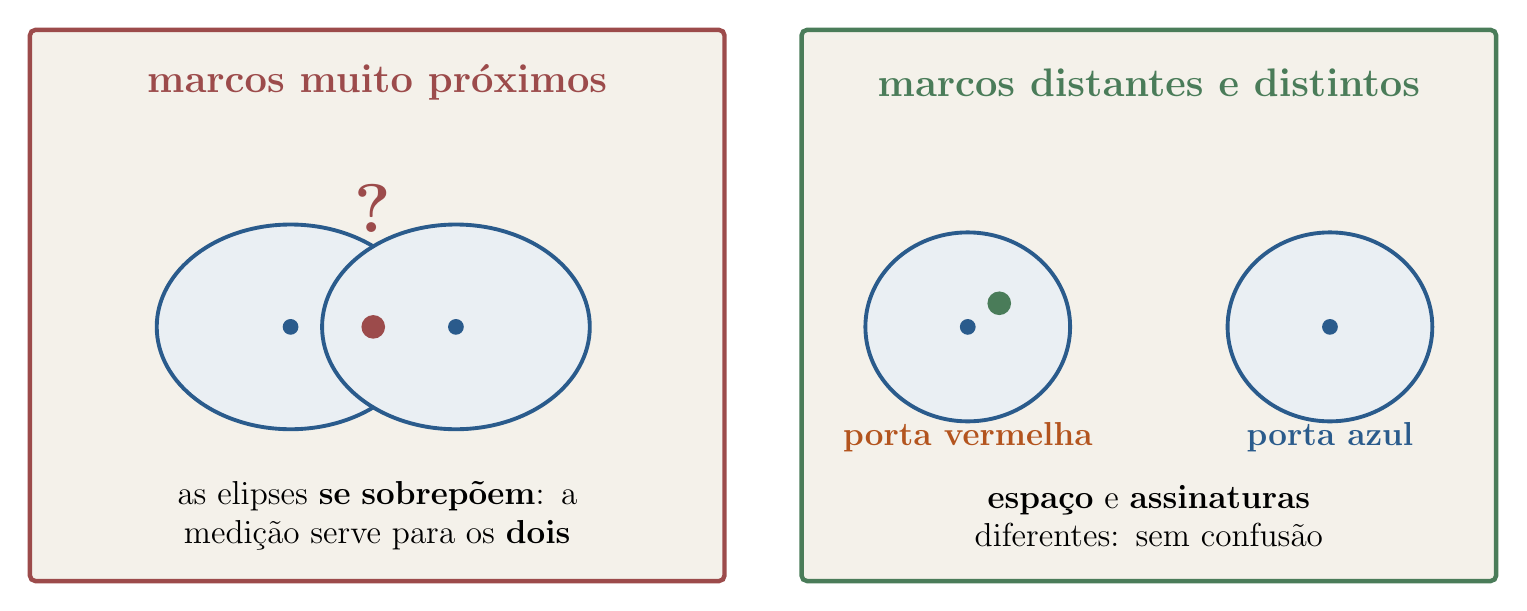
\begin{tikzpicture}[x=1cm,y=1cm]
\tikzset{c/.style={dbox, text width=8.4cm, minimum height=7.0cm, line width=1.6pt, font=\large, anchor=north},
        e/.style={dblue, fill=dblue!10, line width=1.4pt}}
\node[c, draw=dred] at (4.6,8.2) {};
\node[font=\Large\bfseries, dred] at (4.6,7.5) {marcos muito próximos};
\draw[e] (3.5,4.4) ellipse (1.7 and 1.3); \fill[dblue] (3.5,4.4) circle (0.1);
\draw[e] (5.6,4.4) ellipse (1.7 and 1.3); \fill[dblue] (5.6,4.4) circle (0.1);
\fill[dred] (4.55,4.4) circle (0.15); \node[font=\Huge\bfseries, dred] at (4.55,5.9) {?};
\node[font=\large, text width=7.4cm, align=center] at (4.6,2.0) {as elipses \textbf{se sobrepõem}: a medição serve para os \textbf{dois}};
\node[c, draw=dgreen] at (14.4,8.2) {};
\node[font=\Large\bfseries, dgreen] at (14.4,7.5) {marcos distantes e distintos};
\draw[e] (12.1,4.4) ellipse (1.3 and 1.2); \fill[dblue] (12.1,4.4) circle (0.1);
\draw[e] (16.7,4.4) ellipse (1.3 and 1.2); \fill[dblue] (16.7,4.4) circle (0.1);
\fill[dgreen] (12.5,4.7) circle (0.15);
\node[font=\large\bfseries, dorange] at (12.1,3.0) {porta vermelha};
\node[font=\large\bfseries, dblue] at (16.7,3.0) {porta azul};
\node[font=\large, text width=7.4cm, align=center] at (14.4,2.0) {\textbf{espaço} e \textbf{assinaturas} diferentes: sem confusão};
\end{tikzpicture}
\end{document}
